\section{Object manager}
{\bf Part 2 chapter 8}

The object manager responsible for creating, deleting, protecting, and tracking Windows executive objects and abstract data types that are used to represent OS resources such as processes, threads, and the various synchronization objects.
\begin{itemize}
    \item Sysinternals WinObj
    \item Process Explorer
    \item Sysinternals Handle
    \item Ressource Monitor
    \item Kernel debugger \verb+!handle+
\end{itemize}


\subsection{Object types}
three primary types of objects: 
\begin{itemize}
    \item executive objects: are objects implemented by various components of the executive
    \item kernel objects: not visible to user-mode code, provide fundamental capabilities such as synchronization on which executive objects are built (execuive objects encapsulate one or more kernel objects).
    \item GDI/ User objects: belong to windows subsystem and no not interact with kernel
\end{itemize}


\begin{itemize}
    \item the kernel maintains a list of all types of objects it supports.
    \item types have different supported operations and security properties
    \item \verb+Get-NtType+ 
\end{itemize}

\subsection{Object manager namespace (OMNS)}
\begin{verbatim}
    Get-ChildItem NtObject:\ | Sort-Object Name
    Get-ChildItem NtObject:\Dfs | Sort-Object Name
\end{verbatim}

The {\bf Primary Namespace} in Windows Object Manager refers to the main, global namespace that organizes system objects. It is essentially the root namespace where system objects are created and accessed. The primary namespace serves as the central reference point for all objects that can be accessed or manipulated in the system.

The objects in the primary namespace are globally accessible (subject to security and access control) and are referenced by their object names or handles.

Characteristics of the Primary Namespace:
\begin{itemize}
    \item Global Accessibility: Objects are available throughout the entire system.
    \item Well-Known Object Types: 
    \item Access Control: Access control mechanisms (like ACLs and security descriptors) are used to govern which processes can access objects in the primary namespace.
\end{itemize}

The {\bf Secondary Namespace} in the Windows Object Manager refers to a set of namespaces that are used for organizing objects in a more specific context or scope. hese namespaces are typically created for particular subsystems, applications, or kernel components that need to isolate or manage objects within their own boundaries.



Characteristics of the Secondary Namespace:
\begin{itemize}
    \item Specialized Scope: are usually specific to a particular subsystem or context, and they are isolated from the primary namespace
    \item Restricted Access: Objects might not be accessible by all processes. The access to secondary namespace objects can be more restricted, and processes might need to explicitly request access.
    \item Namespacing for Isolation: Secondary namespaces provide a way to logically isolate objects so that different applications or subsystems can have their own namespaces and avoid conflicts or unintended access to one another’s objects.
\end{itemize}


Examples of Secondary Namespace Objects:
\begin{itemize}
    \item Windows Registry:
    \item Security Objects: The Security namespace is another example, where security-related objects (like access tokens, privileges, and security descriptors) are organized and managed.
    \item Process Namespace: Each running process in Windows can have its own namespace for objects such as memory space, threads, and resources.
    \item Device Namespace
\end{itemize}

\subsection{Executive Objects}

Each Windows environment subsystem projects to its applications a different image of the operating
system. The executive objects and object services are primitives that the environment subsystems use
to construct their own versions of objects and other resources

Executive objects are typically created either by an environment subsystem on behalf of a user application or by variuous componets of the OS as part of their normal operation.

The Windows subsystem uses executive objects to export its own set of objects, many of which correspond directly to executive objects.


\subsection{Object structure}

\begin{itemize}
    \item The object manager controls the object headers and footer
    \item The executive components control the object body and type
\end{itemize}

\begin{figure}[!ht]
    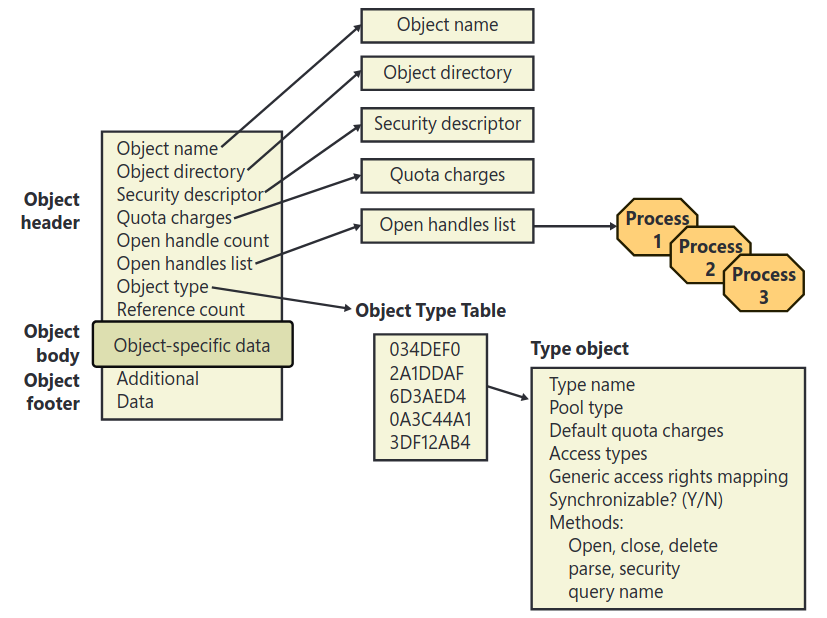
\includegraphics[width=\linewidth]{knowledge/internals/images/obj_structure.png}
    \caption{object structure}
    \label{fig:windows_object_structure}
\end{figure}

the object \verb+type object+ contains info common to each instance.

Additionally, up to eight optional subheaders exist: The name information header, the quota information header, the process information header, the handle information header, the audit information header, the padding information header, the extended information header, and the cre ator information header. 

If the extended information header is present, this means that the object has a footer, and the header will contain a pointer to it.

In addition to the object header, which contains information that applies to any kind of object, the subheaders contains optionalinformation regarding specific aspects ot he object. Note that these  structures are located at a variable offset from the start of the object header, the value of which depends on the number of subheaders associated with the main object header (except creator info).


{\bf windows internals part 2 chapter 8 page 131}

\subsection{Object methods}

{\bf windows internals part 2 chapter 8 page 140}

\subsubsection{Security method}
When an executive component defining an object doesn’t want to override the SRM’s default security policy, it marks the object type as having default security.


An object with default security (mutexes, events, semaphores) stores its security information in its header, and its security method is \verb+SeDefaultObjectMethod+

An object that doesn’t rely on default security must manage its own security information and supply a specific
security method.

A file object is an example of an object that overrides default security. The I/O manager, which defines the file object type, has the file system driver on which a file resides manage (or choose not to implement) the security for its files. Thus, when the system queries the security on a file object that represents a file on an NTFS volume, the I/O manager file object security method retrieves the file’s security using the NTFS file system driver

\subsection{Object handles and the process handle table}

{\bf windows internals part 2 chapter 8 page 143}

Each process object in the kernel has an {\bf handle table} containing:
\begin{itemize}
    \item the handle's numeric identifier
    \item the granted access to the handle
    \item the pointer to the object structure in kernel memory
\end{itemize}

